%!TEX root = thesis.tex

%
%==========================================================================================
%
\chapter{Behavior Signatures}
\label{chap:signatures}

\index{behavior signature}
This chapter discusses how to encode a sequence of actions into a behavior signature. It introduces a novel presentation denoted as a spatio-activity matrix, demonstrates a  visualization technique, and proposes a feature extraction approach.

%
%==========================================================================================
%
\section{Definitions}
In Chapter~\ref{chap:activity_recognition}, we transformed a sequence of observation vectors to a higher-level description of behavior primitives. This chapter discusses how to efficiently encode the sequence of behavior primitives in order to perform additional analysis and effectively visualize the data. By effective visualization, we aim at a presentation that allows humans to quickly compare various behavior patterns and to find the main differences among them.

First, we define static points in the environment that refer to significant locations, specific spatial areas, or regions of partitioned space (for example, squared partitioning).
\begin{definition}
\label{def:landmark}
\index{static landmark}
	\emph{Static landmark} $s$ is a point in the environment that remains fixed over the observed period of time. A set of static landmarks in the environment is denoted as $\mathbb{S}=\{s_i\}$.
\end{definition}
\noindent 

Next, given a set of static landmarks $\mathbb{S}$ and a set of activities $\mathbb{A}$, the behavior can be described in landmark-activity state space $\mathbb{S} \times \mathbb{A}$.
The behavior can be then represented as a trajectory through the landmark-action state space as follows. 

\begin{definition}
\label{def:behavior_trace}
\index{behavior trace}
	\emph{Behavior trace} $\mathbf{b}=\{\tuple{a, s}_t\}, 1 \leq t \leq T$ is a sequence of tuples in which each tuple $\tuple{a,s}_t$ indicates the environmental state $s$ and the activity $a$ being performed at this state at time step $t$.
\end{definition}




%
%==========================================================================================
%

\section{Spatio-Activity Matrix}

\index{feature extraction}
This section introduces a behavior-trace encoding that captures activity distributions, landmark distribution, distribution of activities over landmarks, and distribution of landmarks over activities. 

Consider a set $\mathbb{A}=\{a_1, a_2, ..., a_M\}$ of predefined activities and a set $\mathbb{S}=\{s_1, s_2, ..., s_K\}$ of static landmarks where the agent can be present. Let $\mathbf{v}_t$ denote a spatio-activity vector of size $M+K$ at time step $t$. The first $M$ elements correspond to $M$ activities in $\mathbb{A}$ and the last $K$ elements correspond to static landmarks in $\mathbb{S}$; that is, $i$-th element corresponds to $a_i$ if $i\leq M$ or $s_{i-M}$ if $M < i \leq K$. 

A tuple $(a, s)_t$ is then transformed to the spatio-activity vector with Equation~(\ref{eq:spatio-activity-vector}), which assigns a binary value to $i$-th element of the vector: 1, if the activity is equal to $i$-th activity in $\mathbb{A}$ or if the landmark is equal to landmark at position $i-M$ in $\mathbb{S}$; 0, otherwise.
\begin{equation}
\label{eq:spatio-activity-vector}
\index{spatio-activity matrix}
\mathbf{v}_{t(i)} = \left\{
\begin{array}{l l}
 1 & \quad ;\mbox{if } a=a_i, 1 < i \leq M \mbox{ or } s=s_{i-M}, M < i \leq K,\\
 0 & \quad ;\mbox{otherwise.}\\ \end{array} \right. \
\end{equation}
\noindent A spatio-activity vector is basically a binary representation of activities and landmarks present in a tuple.

Suppose we have two spatio-activity vectors $\mathbf{v}_i$ and $\mathbf{v}_j$. Let $\mathbf{t}(\mathbf{v}_i, \mathbf{v}_j)$ denote a transition vector from the spatio-activity vector $\mathbf{v}_i$ to $\mathbf{v}_j$ as an indication of a change constrained by $\|\mathbf{t}(\mathbf{v}_i, \mathbf{v}_j)\|=1$:
\begin{equation}
\mathbf{t}(\mathbf{v}_i, \mathbf{v}_j) = \neg(\mathbf{v}_j \rightarrow \mathbf{v}_i),
\label{eq:transition}
\end{equation}
\noindent
where operator `$\rightarrow$' is binary implication and `$\neg$' is binary negation.

Now suppose we want to encode the behavior trace $\mathbf{b} = \{(a,s)_t\}, 1 \leq t \leq T$. First, we assign a new vector $\mathbf{v}_t$ to each tuple $(a,s)_t$. Let $\mathbf{M}(\mathbf{b})$ denote the spatio-activity matrix, where the dynamics of a person in the given behavior trace $\mathbf{b}$ is captured:
\begin{equation}
\mathbf{M}(\mathbf{b}) = \mathbf{v}_1  {\mathbf{v}_1}^\intercal + \sum_{t\in[2, ..., T]} [\mathbf{v}_t {\mathbf{v}_t}^\intercal + \mathbf{t}(\mathbf{v}_{t-1}, \mathbf{v}_t) \mathbf{t}(\mathbf{v}_{t-1}, \mathbf{v}_t)^\intercal]
\label{eq:matrix}.
\end{equation}
\noindent
At this step, the spatio-activity matrix $\mathbf{M}$ registered element frequency in a spatio-activity vector and their transitions. In order to make $\mathbf{M}$ comparable to other matrices constructed from behavior traces of different lengths, the matrix $\mathbf{M}$ must be normalized.

Define $norm(\mathbf{M})$ as an operation that normalizes the values of the matrix $\mathbf{M}$ to the interval $[0, 1]$. The $norm(\mathbf{M})$ is defined for an element $\mathbf{M}_{i,j} \in \mathbf{M}$ by the expression
%
\begin{equation}
\mathbf{M}_{i, j} =  \left\{
\begin{array}{l l}

 \frac{\mathbf{M}_{i,j}}{\sum_{k=1}^{M} \mathbf{M}_{k,k}} & ; i = j \wedge i \leq M  \\

 \frac{\mathbf{M}_{i,j}}{\sum_{k=M+1}^{M+K} \mathbf{M}_{k,k}} & ; i = j \wedge i > M  \\

 \frac{\mathbf{M}_{i,j}}{\sum_{\substack{k=1\\l=1\\l\not = k}}^{M} \mathbf{M}_{k,l}} & ; i \neq j \wedge i \leq M \wedge j \leq M  \\

 \frac{\mathbf{M}_{i,j}}{\sum_{\substack{k=M+1\\l=M+1\\l\not = k}}^{M+K} \mathbf{M}_{k,l}} & ; i \neq j \wedge i > M \wedge j > M  \\

 \frac{\mathbf{M}_{i,j}}{\sum_{k=M+1}^{M+K} \mathbf{M}_{i,k}} & ; i \leq M \wedge j > M  \\

 \frac{\mathbf{M}_{i,j}}{\sum_{k=1}^{M} \mathbf{M}_{i,k}} & ; i > M \wedge j \leq M  \\

\end{array}. \right. \
\label{eq:normalize}
\end{equation}
%
Intuitively, the matrix $\mathbf{M}$ consists of six regions as shown in Figure~\ref{fig:matrix-regions}.
\begin{figure}[!ht]
\centering
\includegraphics[width=\textwidth]{chap_BS/matrix}
\caption{Regions of spatio-activity matrix.}
\label{fig:matrix-regions}
\end{figure}
The interpretation of the regions is as follows: the activity-activity part (top left) includes the fractions of the time spent performing particular activities (diagonal elements) and the distribution of transitions between activities (non-diagonal elements); the spatio-spatio part (bottom right) includes the fractions of time spent at the particular landmarks (diagonal elements) and the distribution of transitions  between landmarks (non-diagonal elements); the activity-spatio part (top right) describes the distribution of activities over landmarks; and the spatio-activity part (bottom left) describes the distribution of landmarks over activities.

The complete spatial-activity construction procedure is described in Algorithm~\ref{alg:SA_matrix}. The input is a behavior trace $\mathbf{B}$. Each tuple $(a, s)_t \in \mathbf{B}$ is first transformed into the spatio-activity vector $\mathbf{v}_t$ using Equation~(\ref{eq:spatio-activity-vector}) and added to a temporary sequence of vectors $\mathbf{V}$. The sequence $V$ is then used to compute the spatio-activity matrix $\mathbf{M}$ using Equation~(\ref{eq:matrix}). Finally, the matrix $\mathbf{M}$ is normalized by Equation~(\ref{eq:normalize}).

\begin{algorithm}
\caption{Create spatio-activity matrix.}
\label{alg:SA_matrix}
\begin{algorithmic}
\REQUIRE behavior trace $\mathbf{b}=\{\tuple{a,s}_1,\tuple{a,s}_2,...,\tuple{a,s}_n\}$
\ENSURE normalized matrix $\mathbf{M}(\mathbf{b})$
\STATE $\mathbf{V}\gets \{\}$
\FOR {$\tuple{a,s} \in \mathbf{b}$}
\STATE $\mathbf{v} \gets sa\_vector({\tuple{a,s}}) $
\STATE $\mathbf{V} \gets \mathbf{V} \cup \mathbf{v} $
\ENDFOR
\STATE $\mathbf{M} \gets \mathbf{v}_1  {\mathbf{v}_1}^\intercal$
\FOR {$v_i \in \mathbf{V}$, $i>1$}
 \STATE $\mathbf{M} \gets \mathbf{M} +  \mathbf{v}_i{\mathbf{v}_i}^\intercal + \mathbf{t}_{i-1, i}  {\mathbf{t}_{i, i-1}}^\intercal$
\ENDFOR
%+ \sum_{i\in[1, ..., k]}( v_i*{v_i}^\intercal + t_{i-1, i} * {t_{i, i-1}}^\intercal)$
\STATE $norm(\mathbf{M})$
\end{algorithmic}
\end{algorithm}

%==========================================================================================

\subsection{Time Complexity Analysis}

The runtime complexity increases linearly with the behavior trace length $T$ and quadratically with the sizes of sets $\mathbb{A}$ and $\mathbb{S}$. First, $T(M+K)$ operations are required to transform each tuple to a spatio-activity vector. Next, there are $2(T-1)(M+K)$ operations to compute $T-1$ transition vectors using implication and negation on each pair of spatio-activity vectors. The next step builds the spatio-activity matrix, where each of vector-vector multiplications requires $2(M+K)$ operations that result in matrices. Matrix summarization requires $(M+K)^2$ steps, and is applied for each T. In total there are $2(M+K)+(M+K)^2+T(4(M+K)+(M+K)^2)$ operations. The normalization step can be implemented by pre-computing the six divisors and applying them on each element in the matrix. This requires $T(M+K+M^2+K^2+2(MK))$ operations in total. The overall time complexity, then, is $O(T(M+K)^2)$.

In practice, however, the behavior trace is a few orders of magnitude larger than the number of activities and landmarks; that is, $(M+K) << T$, which makes the computation of spatio-activity matrix dependent only on the behavior trace length $T$.


%==========================================================================================

\subsection{Visualizations}

Since the matrix $\mathbf{M}$ is normalized to the interval $[0, 1]$, it can be visualized with a color map. Figure~\ref{fig:Mmatrix} shows an example of such a matrix $\mathbf{M}$ visualization, where the color ranges from low frequency (blue) to high frequency (red); a warmer color represents a higher intensity (see the legend on the left-hand side). It shows a behavior matrix constructed from a daily behavior trace of a person for activities $\mathbb{A}=\{lying, sitting, standing\}$ and landmarks $\mathbb{S}=\{lounge, bedroom, kitchen, toilet\}$.

\begin{figure}[!ht]
\centering
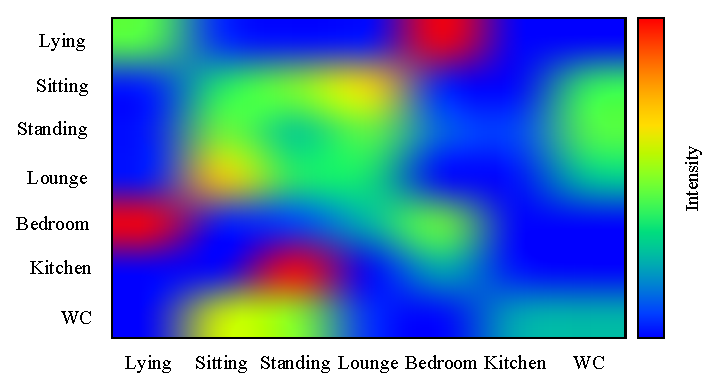
\includegraphics[width=0.9\textwidth]{chap_BS/spatial-activity-matrix}
\caption{Visualization of a daily spatio-activity matrix of one person. A warmer color represents a higher value.}
\label{fig:Mmatrix}
\end{figure}

Figure~\ref{fig:Mmatrix} can be interpreted as follows. There are three red squares that indicate a high ratio: $M_{bedroom, lying}$ indicates that lying is the prevailing bedroom activity;  $M_{kitchen, standing}$ indicates that standing is the prevailing kitchen activity; and $M_{lying, bedroom}$ indicates that lying is mostly carried out in the bedroom. Next, blue squares indicate activity absence; for example, $M_{kitchen, lying}$ and $M_{kitchen, sitting}$ indicate that lying and sitting rarely occurred in the kitchen. Diagonal elements in the bottom-right part of the table (that is, $M_{lounge, lounge}$, $M_{bedroom, bedroom}$, $M_{kitchen, kitchen}$, $M_{toilet, toilet}$) reveal that the person spent most of the time in the bedroom followed by the lounge and toilet, and almost no time in the kitchen.

The visualization is especially useful in a comparison of multiple behavior traces. A small change, for example, in the ratio between sleeping in the bed (being ill) and walking around the apartment (a healthy person), is rapidly propagated through the spatio-activity matrix and, therefore, one can quickly notice the change and the type of change at the same time.


%==========================================================================================

\subsection{Feature Extraction}
\label{sec:ba:PCA}

The behavior matrix can be directly fed into models for anomalous and suspicious behavior detection (discussed in Chapter~\ref{chap:detection}) by transforming the spatio-activity matrix $\mathbf{M}^{M+K, M+K}$ to a feature vector $\mathbf{m}$. Note that the vector $\mathbf{m}$ contains $(M+K)^2$ elements, and some of them rarely change in different behavior traces. The main idea, then, is to reduce the number of features to the most representative set. This section presents an approach based on dimensionality reduction technique denoted as principal component analysis.

\index{principal component analysis}
Principal component analysis (PCA) is an orthogonal linear transformation of possibly correlated variables onto a subspace. The choice of the $k$-dimensional projection subspace is made such that the projection distances have a minimal deformation: squares of the  $k$-dimensional subspace distances are as large as possible. By projecting the data onto the new coordinate system, the greatest variance emerges on the first coordinate (called the first principal component), while the second greatest variance emerges on the second coordinate, and so on.

Implementing PCA is the equivalent of applying Singular Value Decomposition (SVD) to the covariance matrix. Consider a set of spatio-activity matrices $\mathbb{M}=\{\mathbf{M}_i\}$, $1 \leq i \leq L$.
Each spatio-activity matrix $\mathbf{M}_i$ is unrolled into a vector $\mathbf{m}_i$. Then we construct a matrix $\mathbf{\widehat M}$, which consists of $L$ vectors $\mathbf{m}_i$, each unrolled from $\mathbf{M}_i$, $i=1...L$.

\begin{eqnarray}
\mathbf{\widehat M} = \begin{bmatrix}
		\mathbf{m}_1 \\
		\mathbf{m}_2 \\
		\vdots \\
		\mathbf{m}_L \\
	\end{bmatrix} = \begin{bmatrix}
		\mathbf{M}_{1,1} & \mathbf{M}_{1,2} & \cdots & \mathbf{M}_{1, (M+K)^2} & \\
		\mathbf{M}_{2,1} & \mathbf{M}_{2,2} & \cdots & \mathbf{M}_{2, (M+K)^2} & \\
		\vdots 			 &	\vdots			& \ddots & \cdots \\
		\mathbf{M}_{L,1} & \mathbf{M}_{L,2} & \cdots & \mathbf{M}_{L, (M+K)^2} & \\
	\end{bmatrix}
\end{eqnarray}

 The PCA proceeds as follows:  first, we compute the mean vector $\mathbf{\bar\mu}$ with $\mu_j$ elements, $1 \leq j \leq (M+N)^2$ with Equation~(\ref{eq:PCA-1}), and subtract the mean from $\mathbf{\widehat M}$ with Equation~(\ref{eq:PCA-2}), which gives us matrix $\mathbf{\widehat M}_z$ with zero mean.

\begin{equation}
\mu_j = {1 \over L} \sum_{k=1}^L \mathbf{M}_{k, j}, 1 \leq j \leq (M+N)^2
\label{eq:PCA-1}
\end{equation}

\begin{equation}
\mathbf{\widehat M}_z = \mathbf{\widehat M} - \begin{bmatrix}
		1 \\
		1 \\
		\vdots \\
		1 \\
	\end{bmatrix}_{L} \mathbf{\bar\mu}
\label{eq:PCA-2}
\end{equation}

Next, a matrix $\mathbf{C}$ of variances and covariances is computed with Equation~(\ref{eq:PCA-3}), where the diagonal elements $i = j$ are variances $\sigma_{ij}^2$ and the non-diagonal elements $i \neq j$ are covariances $\sigma_i\sigma_j$. 

\begin{equation}
\mathbf{C} = {1 \over L} \mathbf{\widehat M}_z \mathbf{\widehat M}_z^\intercal
\label{eq:PCA-3}
\end{equation}

Finally, $\mathbf{C}$ is decomposed into three matrices with SVD (Equation~(\ref{eq:PCA-4})). $\mathbf{S}$ is a diagonal matrix that stores singular values $\lambda_1, \lambda_2, ..., \lambda_n$. $\mathbf{U}$ and $\mathbf{V}$ are orthogonal matrices, while their column vectors are the so-called left and right eigenvectors of $\mathbf{C}$. 

\begin{equation}
\mathbf{C} = \mathbf{USV}^\intercal
\label{eq:PCA-4}
\end{equation}

When these eigenvectors multiply $\mathbf{\widehat M}_z$, the coordinates are shifted and rotated until they end up aligned with basis vectors. Note that PCA now re-expresses the data as a linear combination of its basis vectors, $\mathbf{\widehat M}_z\mathbf{V}$. $\mathbf{V}$ columns are found to produce the desired linear combinations. The first $\mathbf{V}$ column corresponds to the largest principal component, the second column corresponds to the second largest, and so on. These define the direction in which the variability of the original data set is maximized.

The transformed data now enable the use of anomalous and suspicious behavior detection models. All the behavior matrices $\{\mathbf{M}_i\} \in \mathbb{M}$, $1 \leq i \leq L$ are first expressed in the new coordinate system. When a new behavior matrix $\mathbf{M}_{L+1}$ is obtained, it is first expressed in the same system; the first components are subsequently used for further detection.
%As the first method we have chosen Local Outlier Factor algorithm because it has proven successful in several previous projects (literature?).


%
%==========================================================================================
%

\section{Summary and Discussion}
This chapter proposed a novel, efficient encoding denoted as spatio-activity matrix that is able to capture behavior dynamics in a specific time period using spatio-temporal features. We provided a visualization technique to compare different behavior patterns. We further provided a feature extraction technique based on principal component analysis to reduce the spatio-activity matrix dimensionality, which can be directly used in anomaly detection algorithms. Compared to related work based on HMMs~\citep{Monekosso}, the behavior patterns dynamics is expressed explicitly and can be visualized. Moreover, in contrast to research based on rule induction~\citep{Lee04daily,Lymberopoulos}, the presentation does not extract the exact behavior patterns, which leads to better generalization.

The obtained spatio-temporal features or their principal componentes will be used in the next chapter, which evaluates behavior patterns to perform anomalous and suspicious behavior detection. The spatio-temporal matrix can be constructed on various time intervals, such as hours, days, weeks, which provides different behavior encoding granularities; Section~\ref{sec:combine} discusses how to combine such evaluations. Also, the approach was demonstrated on spatio-temporal feature space, but in general, it can be applied on other feature spaces as well, which is an interesting direction for further investigations.

%


% \section{Behavior Trace Visualization}


% %---------------------------------------------------------------------

% \begin{algorithm}
% \caption{Trace visualization.}
% \label{alg:SA_matrix}
% \begin{algorithmic}
% \REQUIRE behavior trace $B=\{(a,s)_1,(a,s)_2,...,(a,s)_n\}$
% \ENSURE normalized matrix $M(B)$
% \STATE $V\gets \{\}$
% \FOR {$e \in S$}
% \STATE $v \gets sa\_vector(e) $
% \STATE $V \gets V \cup v $
% \ENDFOR
% \STATE $M \gets v_1 * {v_1}^\intercal$
% \FOR {$v_i \in V$, $i>1$}
%  \STATE $M \gets M +  v_i*{v_i}^\intercal + t_{i-1, i} * {t_{i, i-1}}^\intercal$
% \ENDFOR
% %+ \sum_{i\in[1, ..., k]}( v_i*{v_i}^\intercal + t_{i-1, i} * {t_{i, i-1}}^\intercal)$
% \STATE $norm(M)$
% \end{algorithmic}
% \end{algorithm}

% \begin{figure}[!ht]
% \centering
% 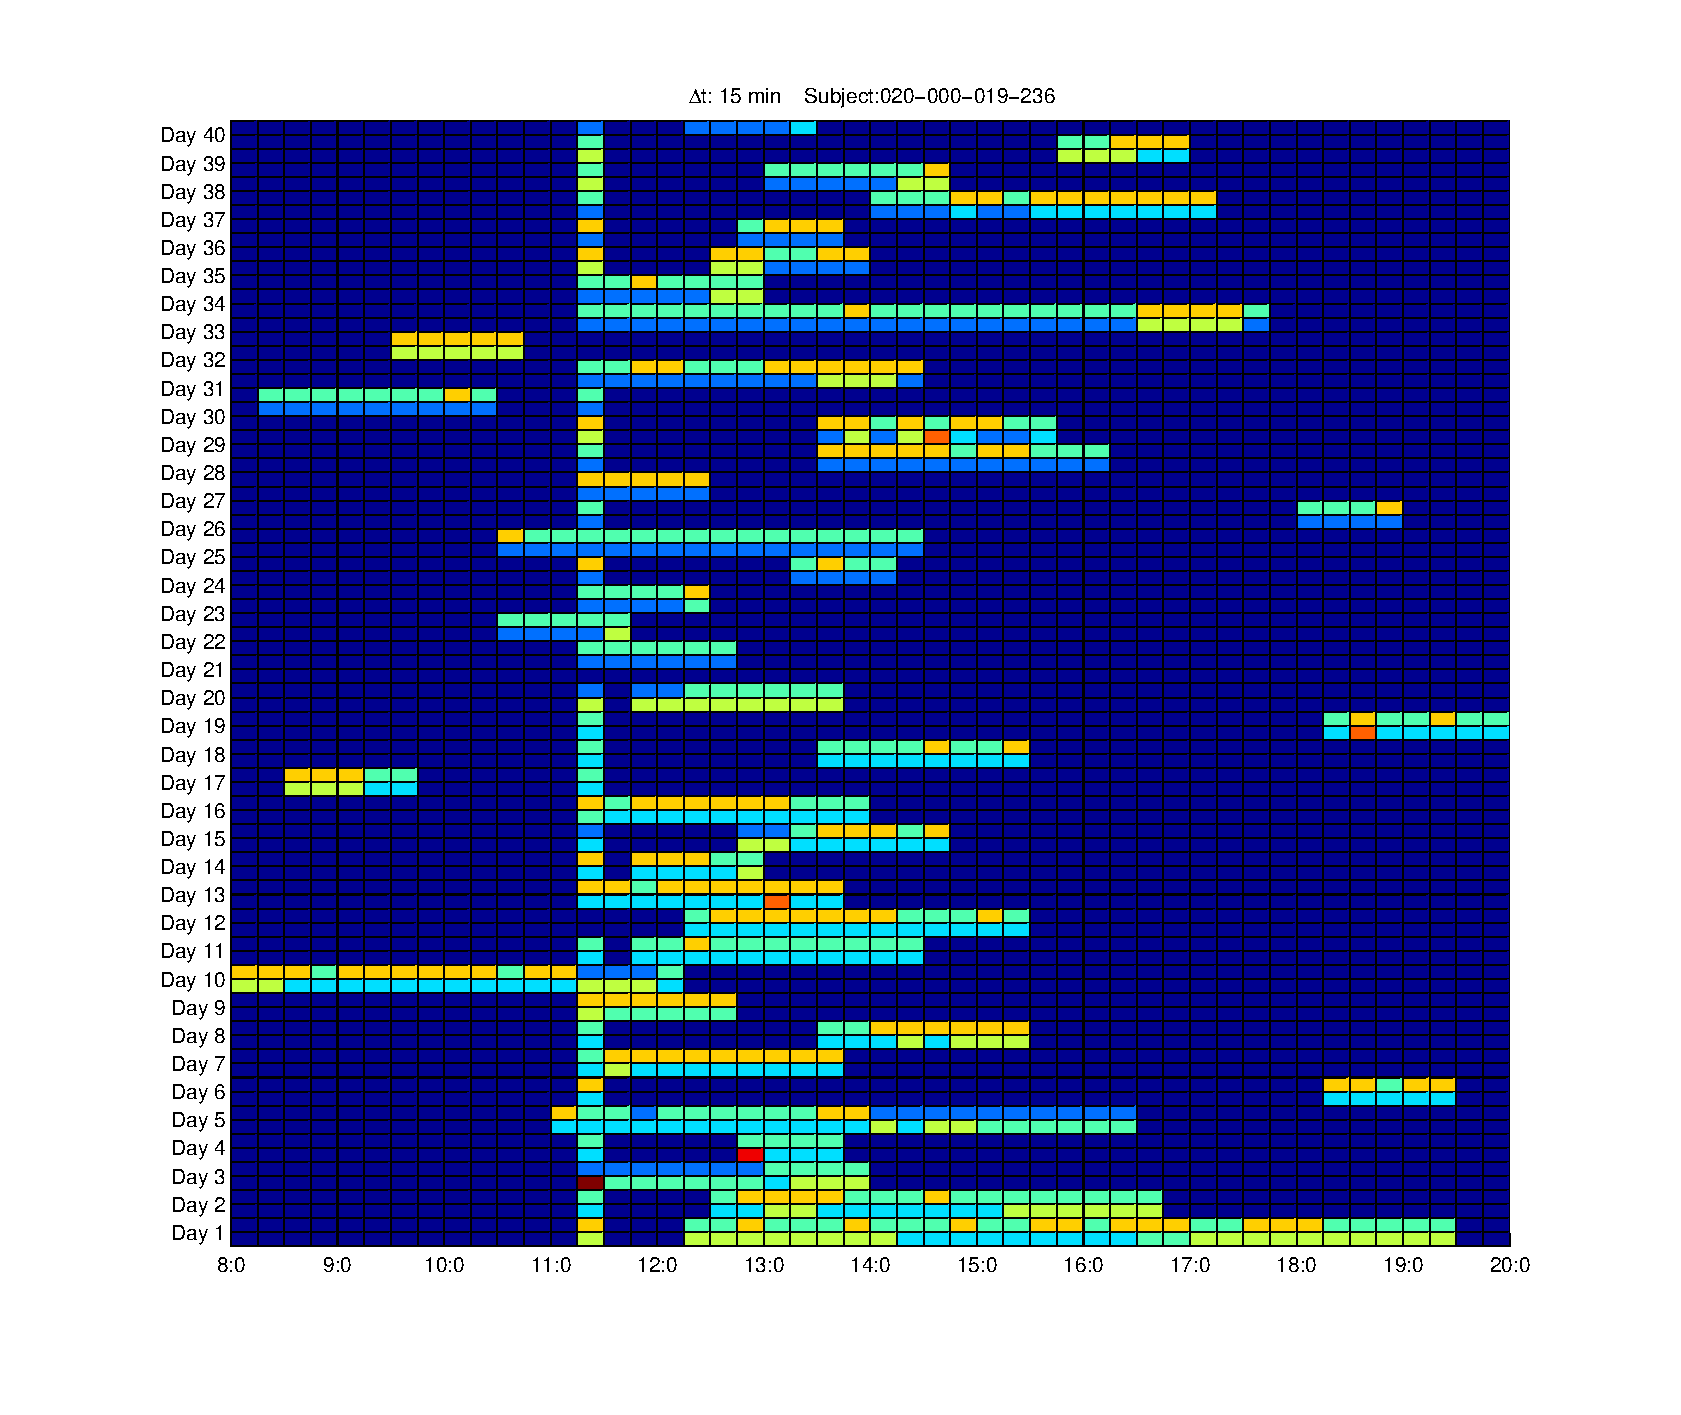
\includegraphics[width=\textwidth]{chap_BS/days}
% \caption{An example of monthly visualization.}
% \label{fig:month-signature}
% \end{figure}

% %---------------------------------------------------------------------

% \begin{algorithm}
% \caption{Behavior trace over time intervals.}
% \label{alg:SA_matrix}
% \begin{algorithmic}
% \REQUIRE behavior trace $B=\{(a,s)_1,(a,s)_2,...,(a,s)_n\}$
% \ENSURE normalized matrix $M(B)$
% \STATE $V\gets \{\}$
% \FOR {$e \in S$}
% \STATE $v \gets sa\_vector(e) $
% \STATE $V \gets V \cup v $
% \ENDFOR
% \STATE $M \gets v_1 * {v_1}^\intercal$
% \FOR {$v_i \in V$, $i>1$}
%  \STATE $M \gets M +  v_i*{v_i}^\intercal + t_{i-1, i} * {t_{i, i-1}}^\intercal$
% \ENDFOR
% %+ \sum_{i\in[1, ..., k]}( v_i*{v_i}^\intercal + t_{i-1, i} * {t_{i, i-1}}^\intercal)$
% \STATE $norm(M)$
% \end{algorithmic}
% \end{algorithm}

% \begin{figure}[!ht]
% \centering
% 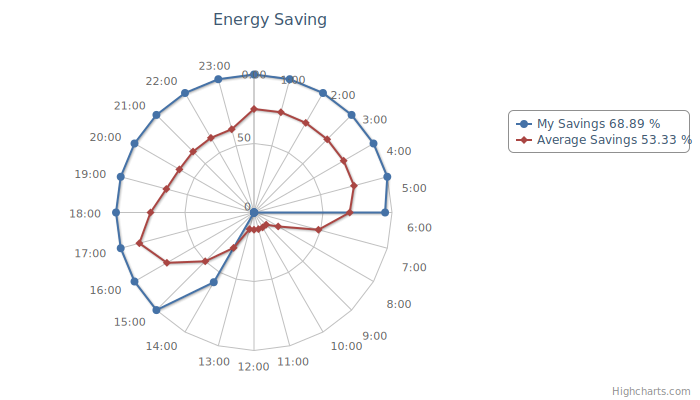
\includegraphics[width=\textwidth]{chap_BS/spider}
% \caption{An example of daily visualization.}
% \label{fig:spider}
% \end{figure}
